\section{Appendix}


% RANDOM ATTACK
\begin{figure}
	\centering
	\begin{subfigure}[b]{0.45\textwidth}
		\centering
		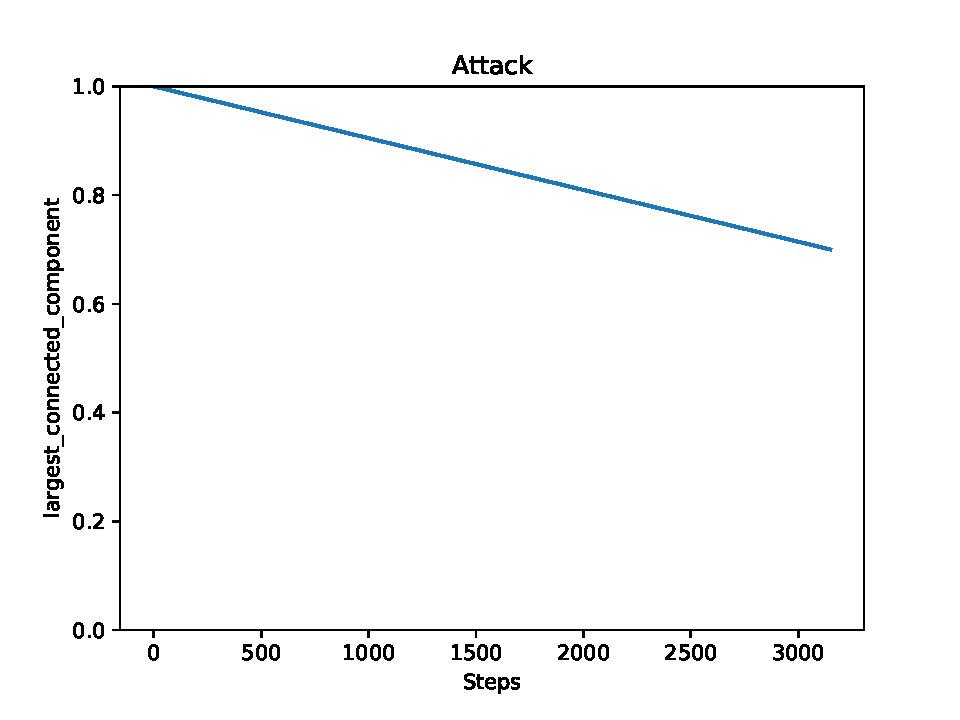
\includegraphics[width=\textwidth]{Images/plots_rnd/rnd_20.pdf}
		\caption{for $10500$ neurons}
		%\label{fig:y equals x}
	\end{subfigure}
	\hfill
	\begin{subfigure}[b]{0.45\textwidth}
		\centering
		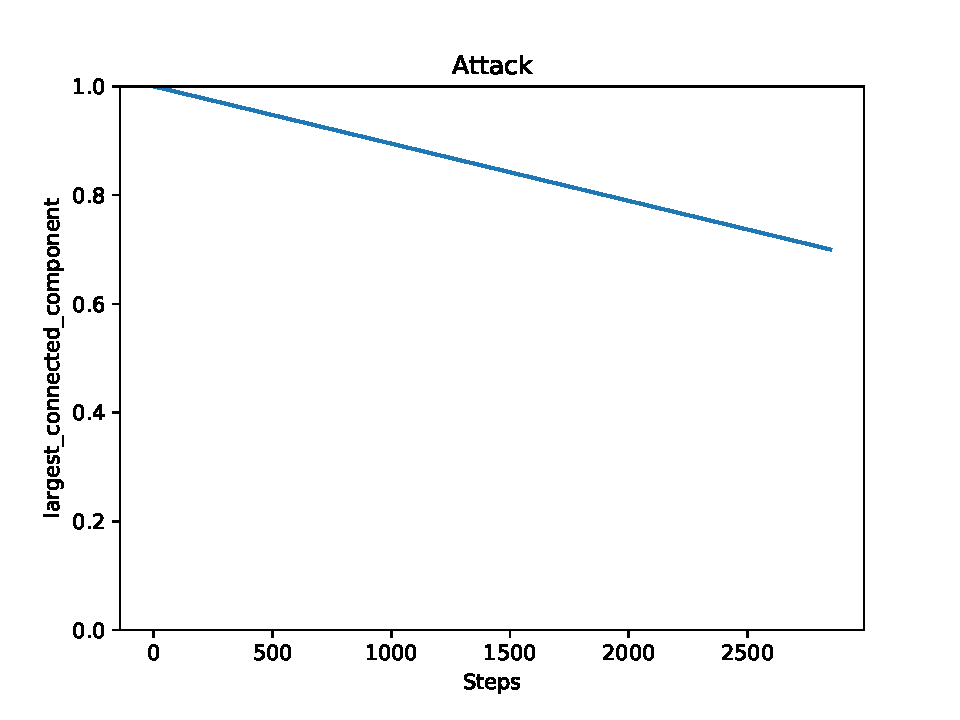
\includegraphics[width=\textwidth]{Images/plots_rnd/rnd_22.pdf}
		\caption{for $9500$ neurons}
		%\label{fig:three sin x}
	\end{subfigure}
	\\ \vspace{5mm}
	\begin{subfigure}[b]{0.45\textwidth}
		\centering
		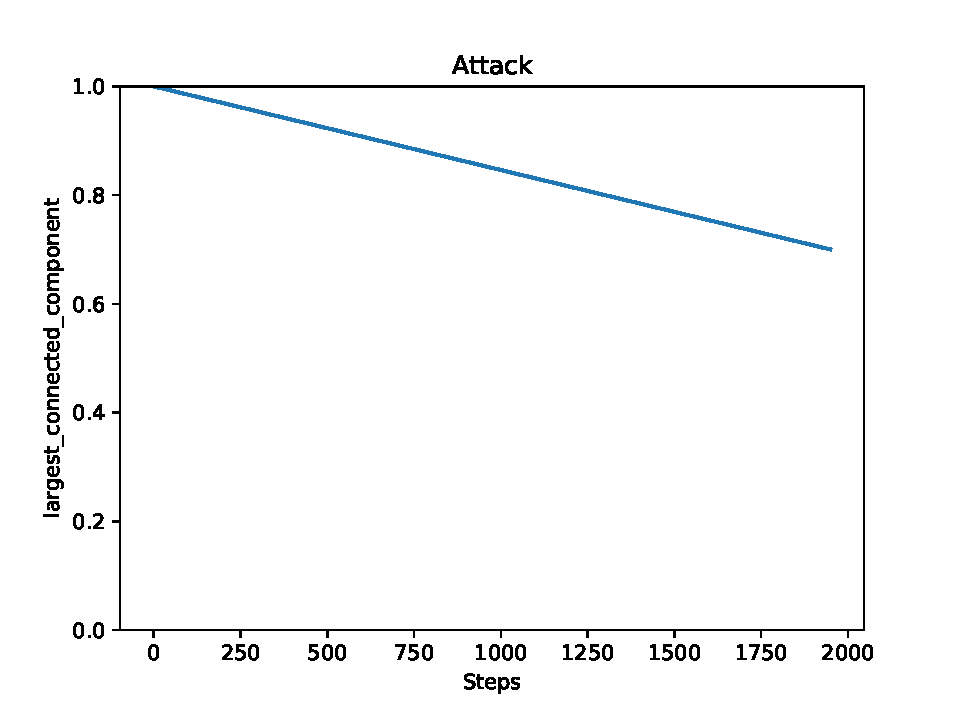
\includegraphics[width=\textwidth]{Images/plots_rnd/rnd_28.pdf}
		\caption{for $6500$ neurons}
		%\label{fig:y equals x}
	\end{subfigure}
	\hfill
	\begin{subfigure}[b]{0.45\textwidth}
		\centering
		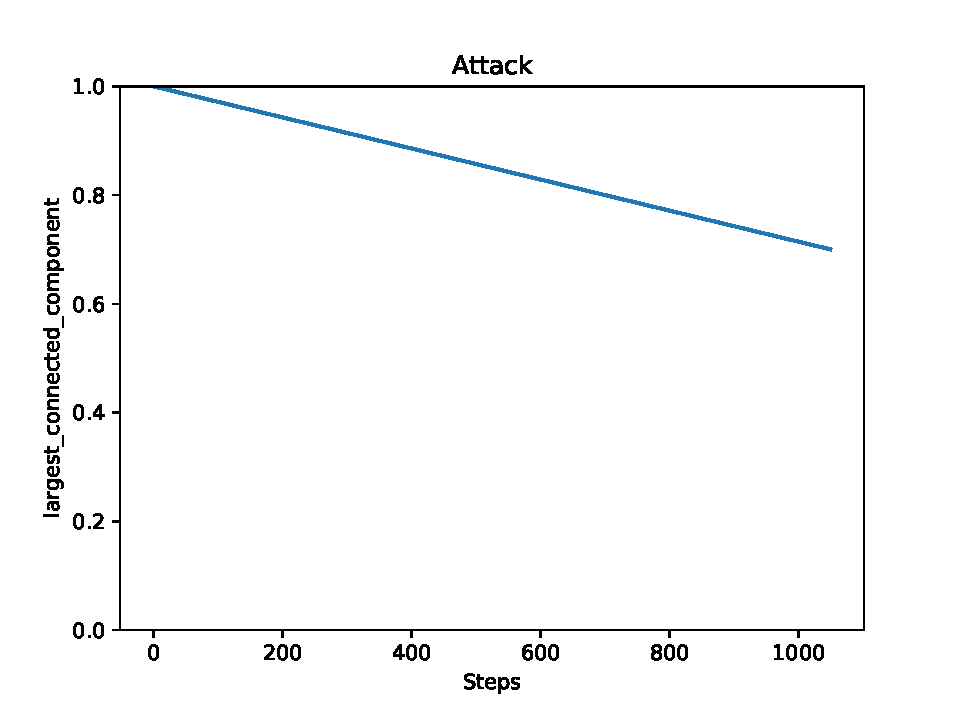
\includegraphics[width=\textwidth]{Images/plots_rnd/rnd_34.pdf}
		\caption{for $3500$ neurons}
		%\label{fig:three sin x}
	\end{subfigure}
	\\ \vspace{5mm}
	\begin{subfigure}[b]{0.45\textwidth}
		\centering
		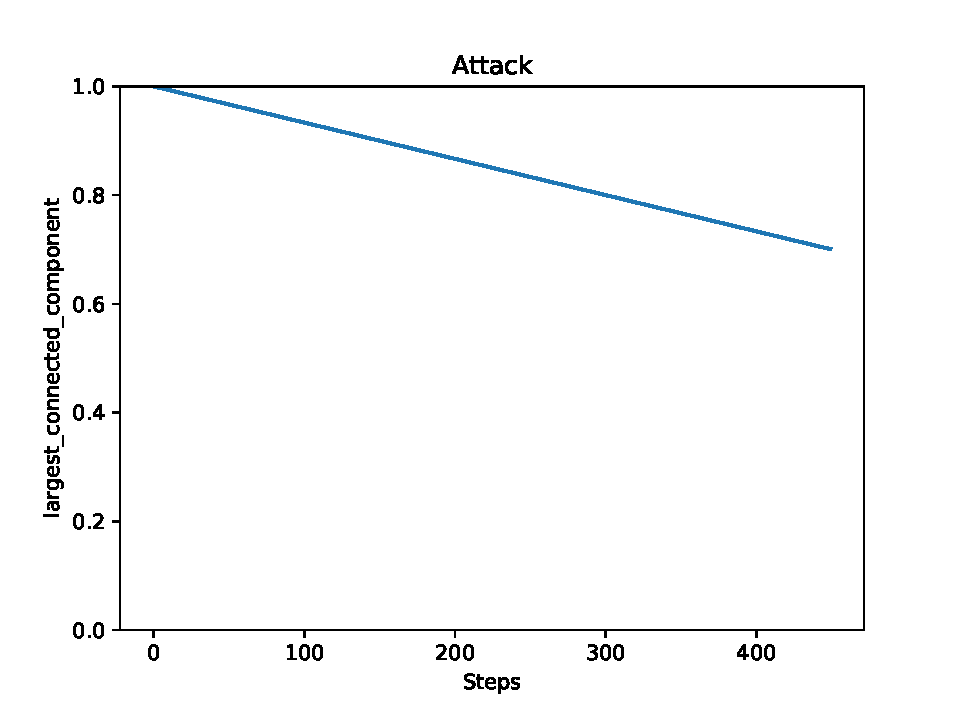
\includegraphics[width=\textwidth]{Images/plots_rnd/rnd_38.pdf}
		\caption{for $1500$ neurons}
		%\label{fig:y equals x}
	\end{subfigure}
	\hfill
	\begin{subfigure}[b]{0.45\textwidth}
		\centering
		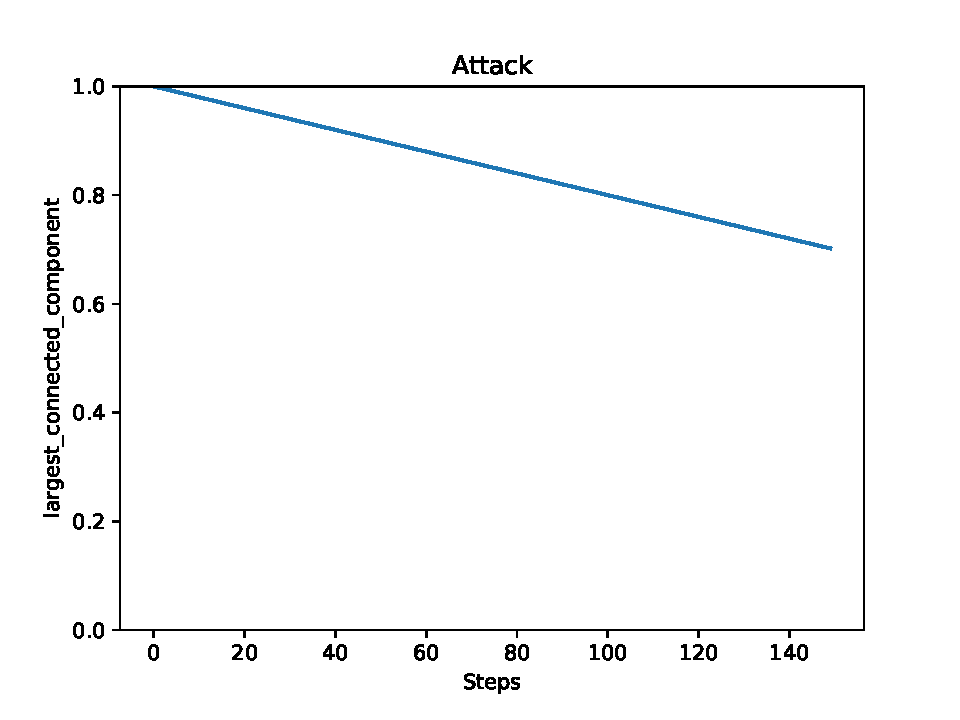
\includegraphics[width=\textwidth]{Images/plots_rnd/rnd_40.pdf}
		\caption{for $500$ neurons}
		%\label{fig:three sin x}
	\end{subfigure}
	\\ \vspace{5mm}
	

	\caption{Robustness of the network at various graining scales against random node removal attacks, using the largest connected component as measure.}
	\label{fig:rnd_atk}
\end{figure}


% BETWEENNESS ATTACK
\begin{figure}
	\centering
	\begin{subfigure}[b]{0.45\textwidth}
		\centering
		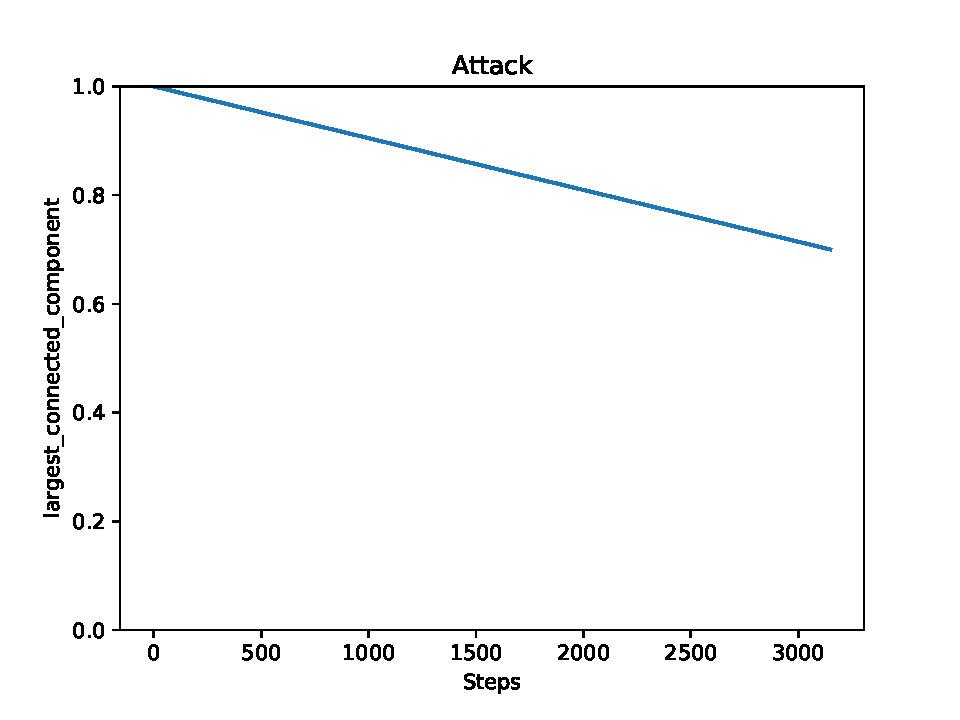
\includegraphics[width=\textwidth]{Images/plots_ib/ib_20.pdf}
		\caption{for $10500$ neurons}
		%\label{fig:y equals x}
	\end{subfigure}
	\hfill
	\begin{subfigure}[b]{0.45\textwidth}
		\centering
		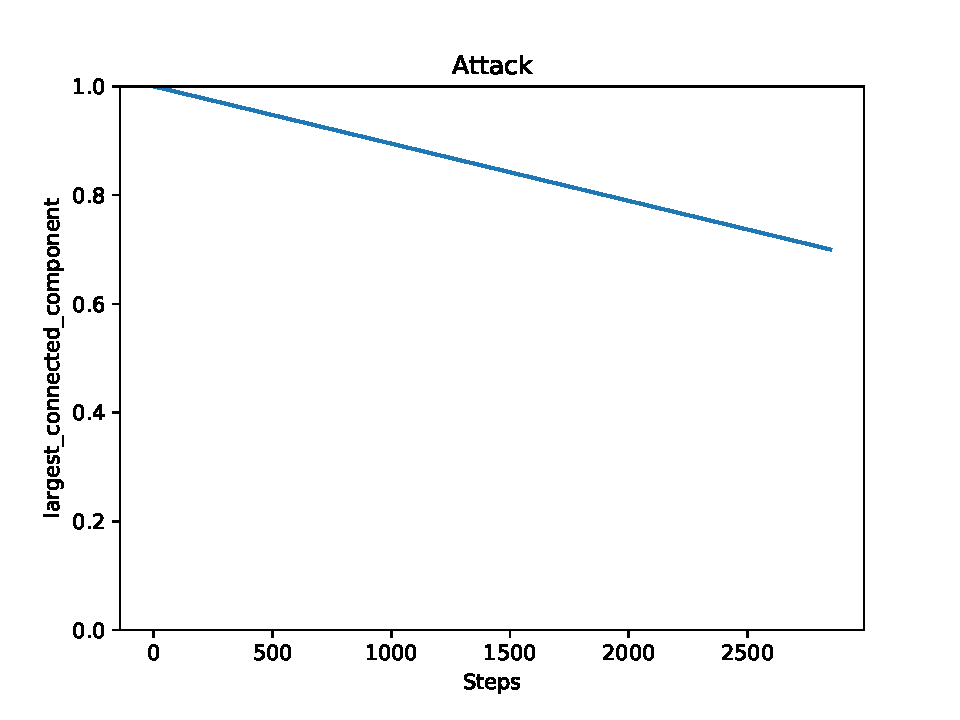
\includegraphics[width=\textwidth]{Images/plots_ib/ib_22.pdf}
		\caption{for $9500$ neurons}
		%\label{fig:three sin x}
	\end{subfigure}
	\\ \vspace{5mm}
	\begin{subfigure}[b]{0.45\textwidth}
		\centering
		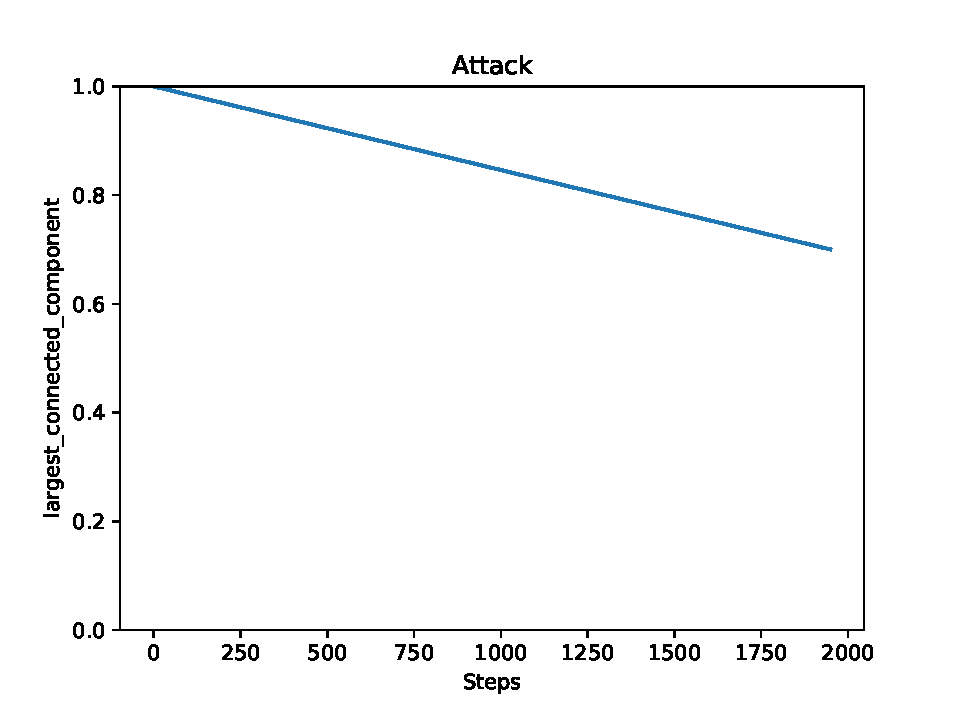
\includegraphics[width=\textwidth]{Images/plots_ib/ib_28.pdf}
		\caption{for $6500$ neurons}
		%\label{fig:y equals x}
	\end{subfigure}
	\hfill
	\begin{subfigure}[b]{0.45\textwidth}
		\centering
		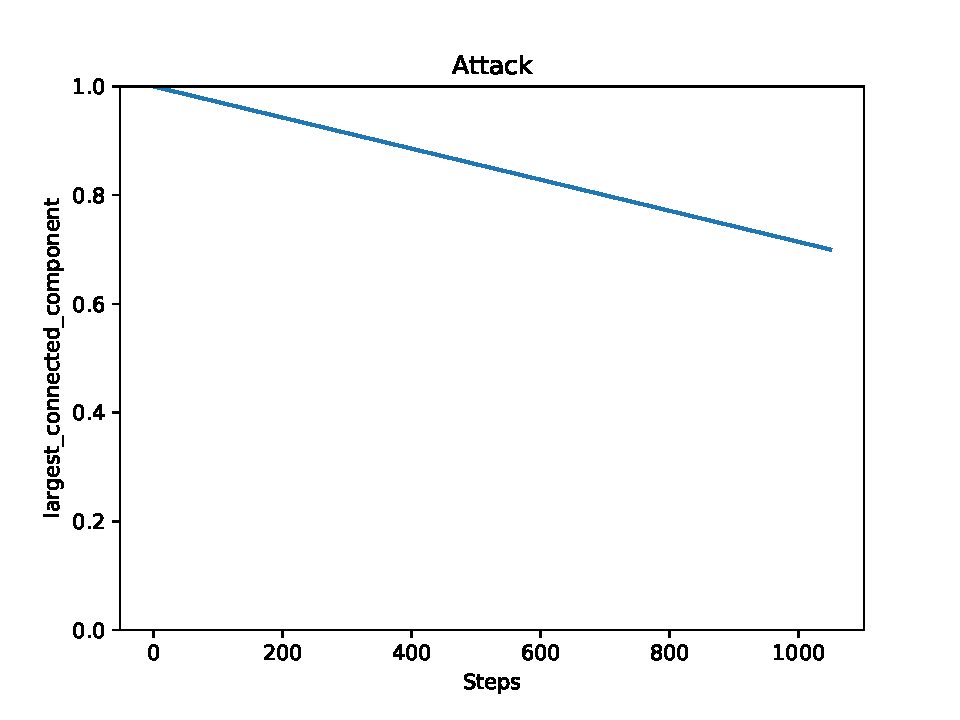
\includegraphics[width=\textwidth]{Images/plots_ib/ib_34.pdf}
		\caption{for $3500$ neurons}
		%\label{fig:three sin x}
	\end{subfigure}
	\\ \vspace{5mm}
	\begin{subfigure}[b]{0.45\textwidth}
		\centering
		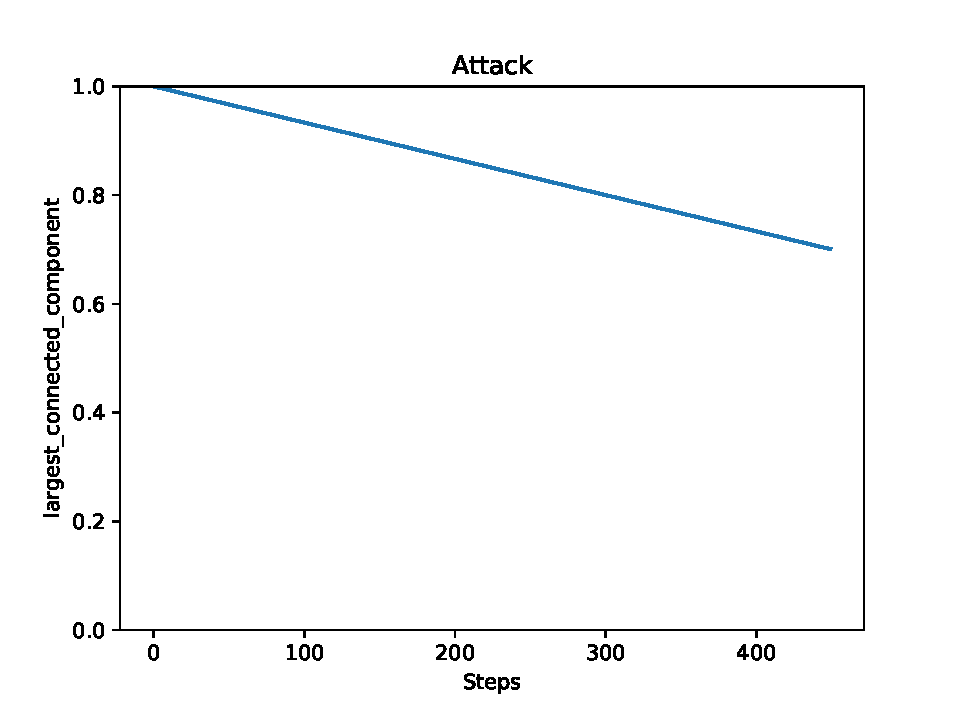
\includegraphics[width=\textwidth]{Images/plots_ib/ib_38.pdf}
		\caption{for $1500$ neurons}
		%\label{fig:y equals x}
	\end{subfigure}
	\hfill
	\begin{subfigure}[b]{0.45\textwidth}
		\centering
		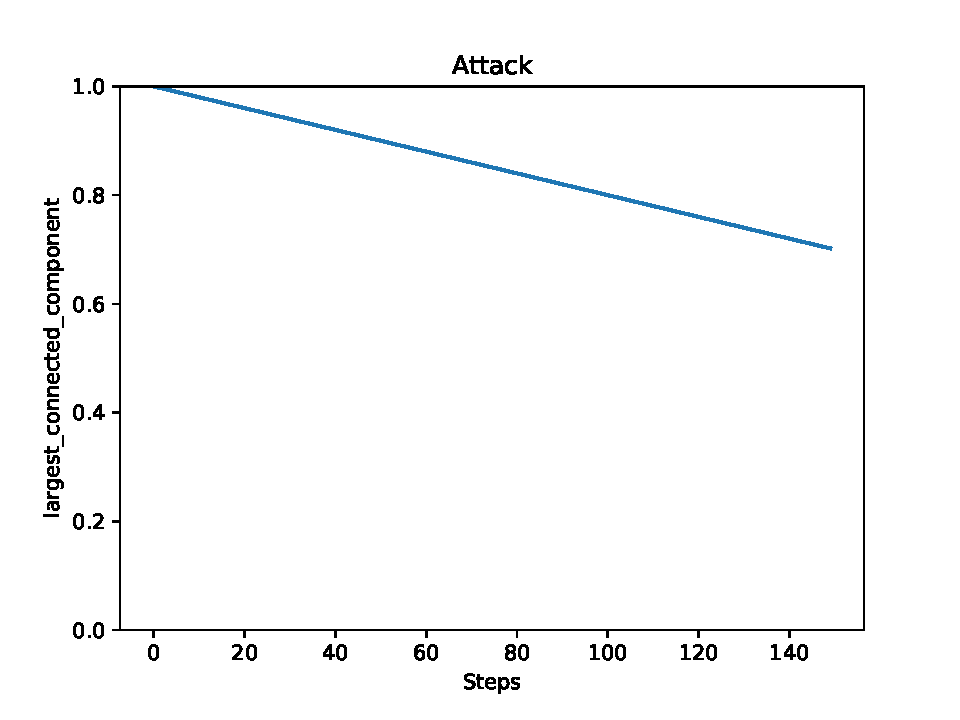
\includegraphics[width=\textwidth]{Images/plots_ib/ib_40.pdf}
		\caption{for $500$ neurons}
		%\label{fig:three sin x}
	\end{subfigure}
	\\ \vspace{5mm}
	
	
	\caption{Robustness of the network at various graining scales against removal of highest-betweenness nodes attack, using the largest connected component as measure.}
	\label{fig:ib_atk}
\end{figure}


% CASCADING ATTACK
\begin{figure}
	\centering
	\begin{subfigure}[b]{0.45\textwidth}
		\centering
		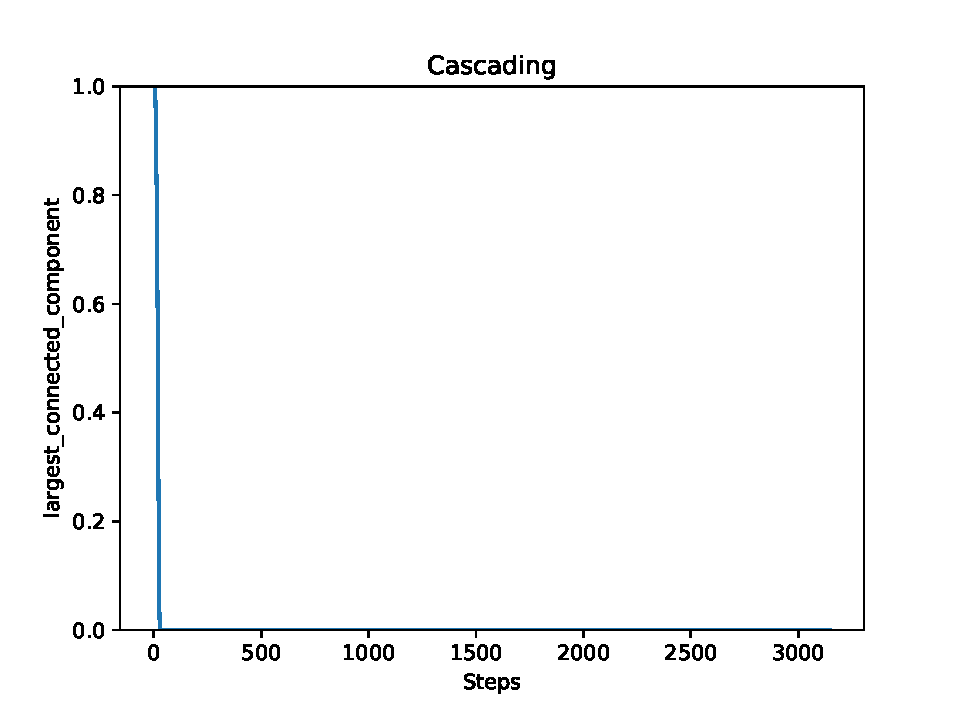
\includegraphics[width=\textwidth]{Images/plots_cascading/cascading_20.pdf}
		\caption{for $10500$ neurons}
		%\label{fig:y equals x}
	\end{subfigure}
	\hfill
	\begin{subfigure}[b]{0.45\textwidth}
		\centering
		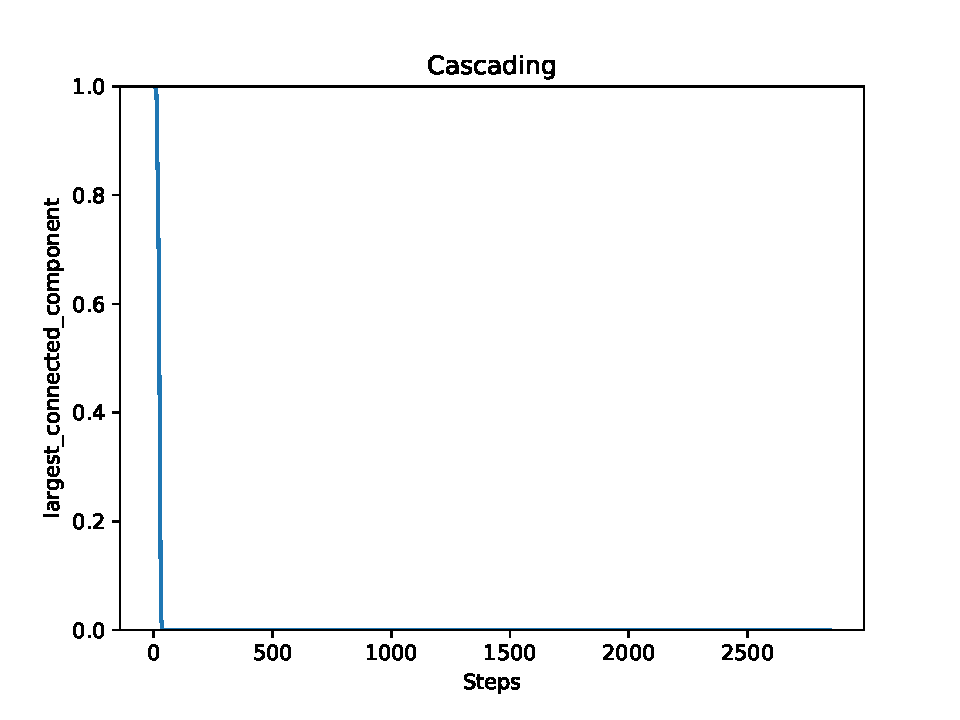
\includegraphics[width=\textwidth]{Images/plots_cascading/cascading_22.pdf}
		\caption{for $9500$ neurons}
		%\label{fig:three sin x}
	\end{subfigure}
	\\ \vspace{5mm}
	\begin{subfigure}[b]{0.45\textwidth}
		\centering
		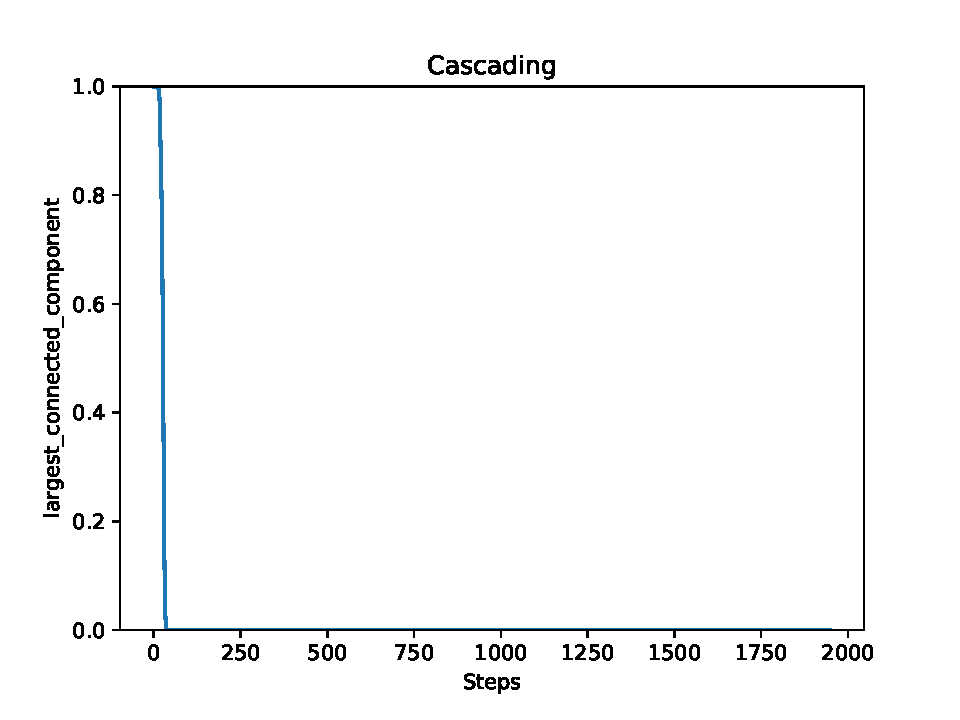
\includegraphics[width=\textwidth]{Images/plots_cascading/cascading_28.pdf}
		\caption{for $6500$ neurons}
		%\label{fig:y equals x}
	\end{subfigure}
	\hfill
	\begin{subfigure}[b]{0.45\textwidth}
		\centering
		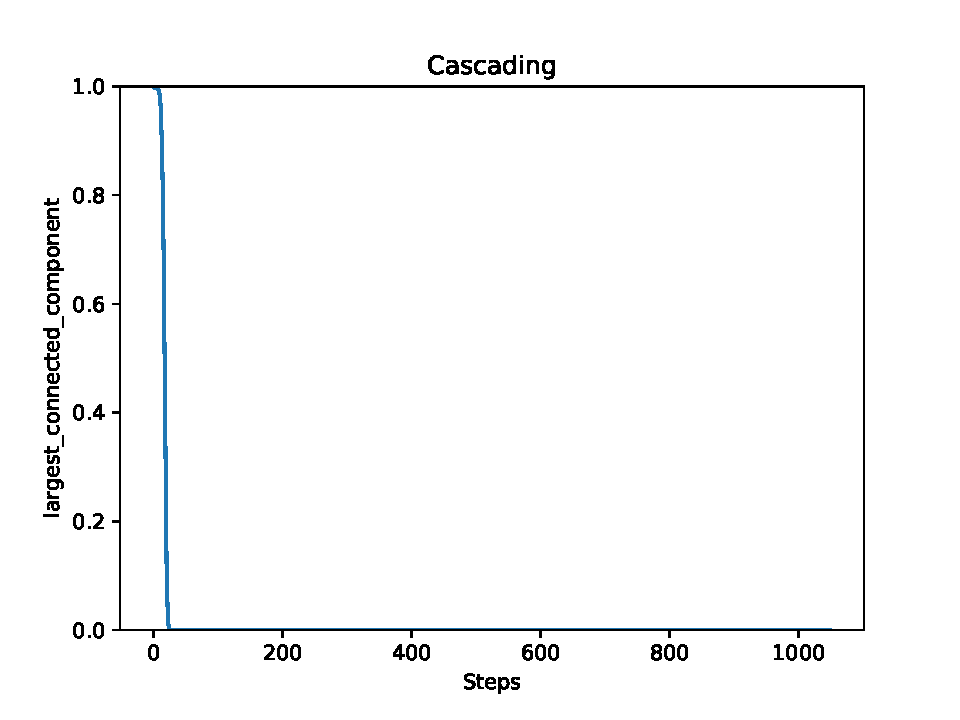
\includegraphics[width=\textwidth]{Images/plots_cascading/cascading_34.pdf}
		\caption{for $3500$ neurons}
		%\label{fig:three sin x}
	\end{subfigure}
	\\ \vspace{5mm}
	\begin{subfigure}[b]{0.45\textwidth}
		\centering
		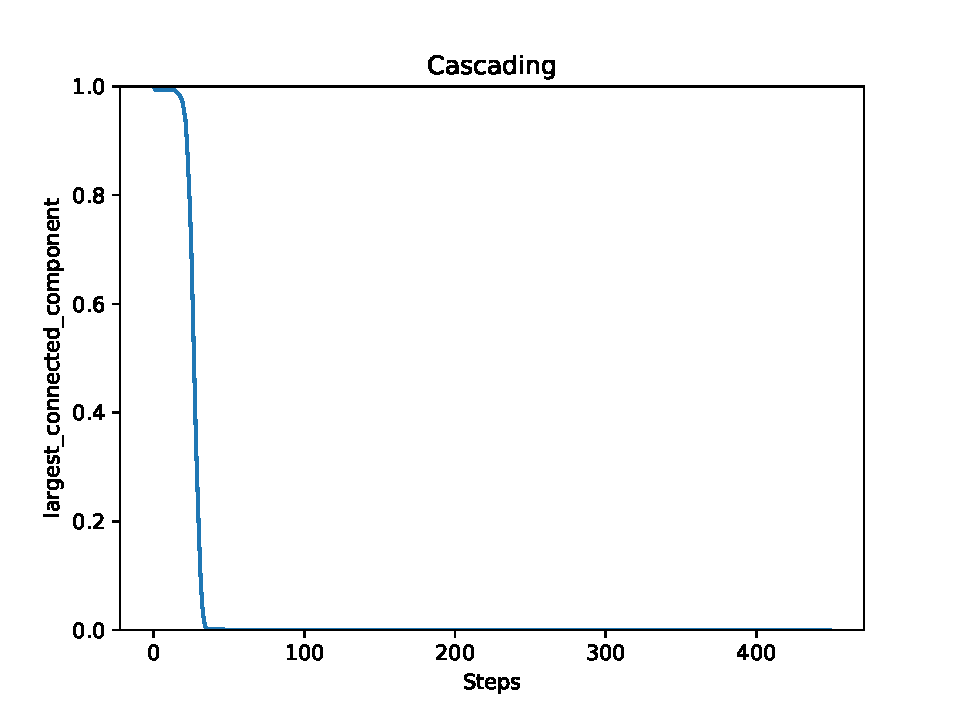
\includegraphics[width=\textwidth]{Images/plots_cascading/cascading_38.pdf}
		\caption{for $1500$ neurons}
		%\label{fig:y equals x}
	\end{subfigure}
	\hfill
	\begin{subfigure}[b]{0.45\textwidth}
		\centering
		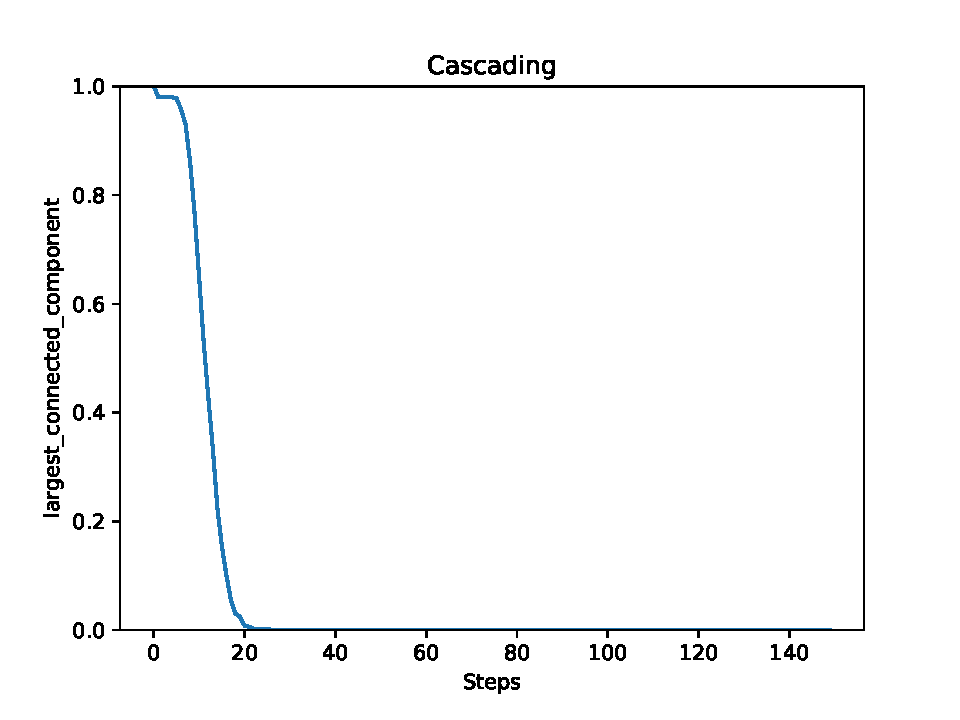
\includegraphics[width=\textwidth]{Images/plots_cascading/cascading_40.pdf}
		\caption{for $500$ neurons}
		%\label{fig:three sin x}
	\end{subfigure}
	\\ \vspace{5mm}
	
	
	\caption{Robustness of the network at various graining scales against removal of highest-betweenness cascading attack, using the largest connected component as measure.}
	\label{fig:cascading_atk}
\end{figure}